\section{}
\[
H(s)=\frac{s^2+2s+10}{s^2+2s+10}=1\,.
\]
\subsection{Bode-Diagramm}
\begin{center}
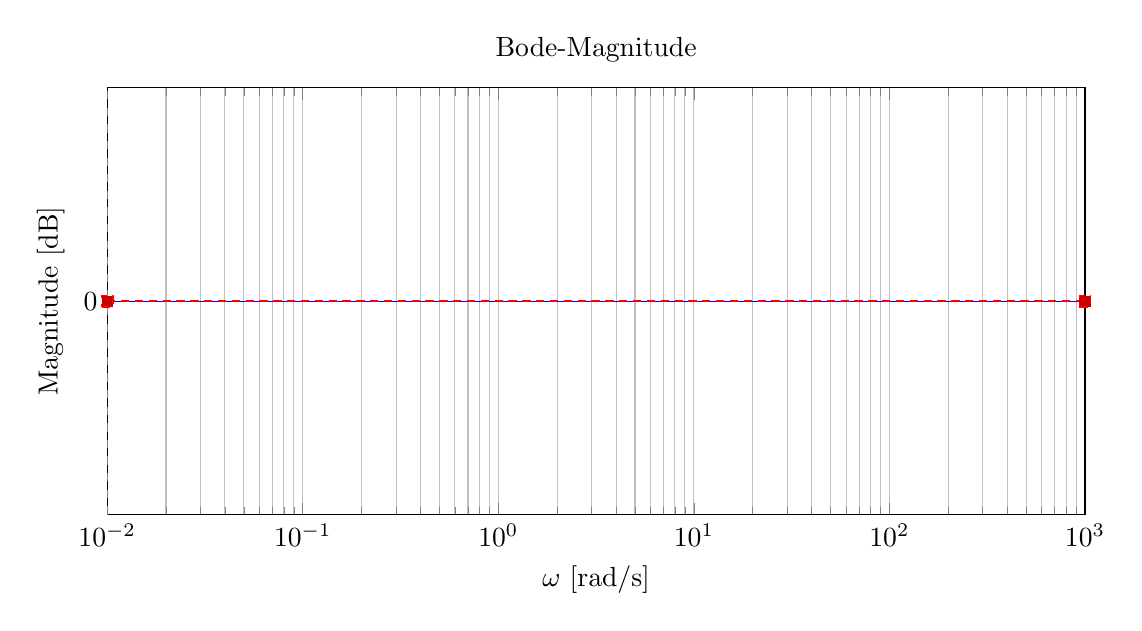
\begin{tikzpicture}
\begin{semilogxaxis}[
  width=14cm,height=7cm,
  xmin=1e-2,xmax=1e3,
  ytick distance=20,
  ytick={-20,0,20},
  xlabel={$\omega$ [rad/s]},
  ylabel={Magnitude [dB]},
  grid=both,
  title={Bode-Magnitude}
]
\addplot[
  domain=1e-2:1e3,
  samples=2,
  mark=none,
  line width=0.3pt,
  blue
] {0};
\addplot+[domain=1e-2:1e3,samples=2,dashed,dash pattern=on 3pt off 2pt,line width=0.6pt,red] {0};
\draw[gray,dashed] (rel axis cs:0,0) -- (rel axis cs:0,1);
\end{semilogxaxis}
\end{tikzpicture}
\vspace{6mm}
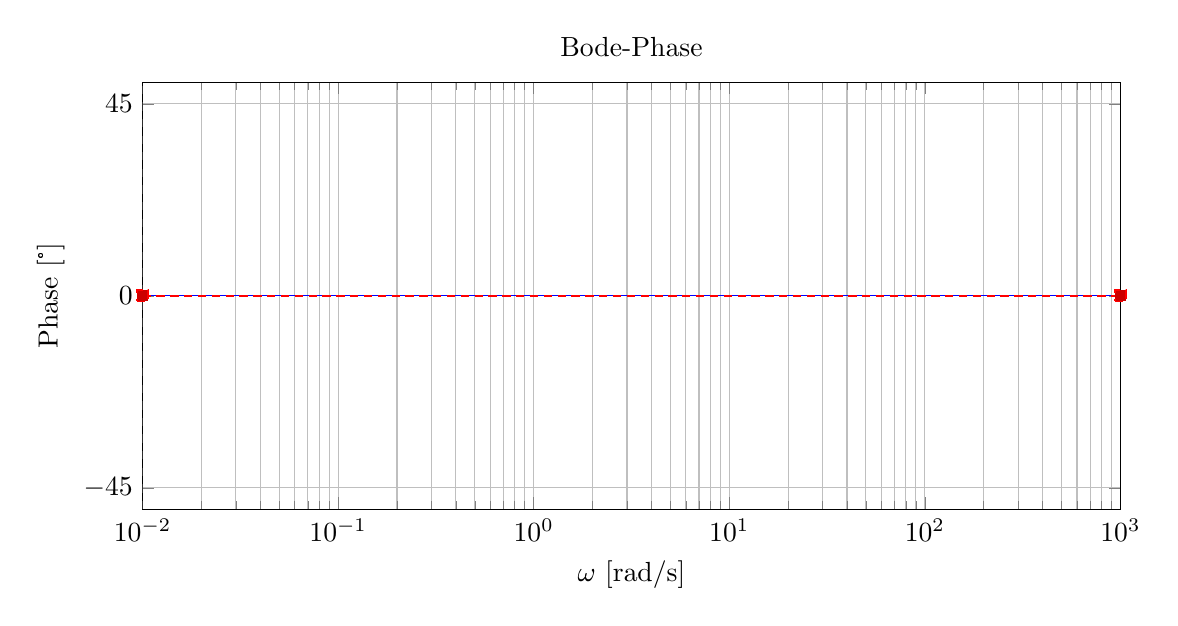
\begin{tikzpicture}
\begin{semilogxaxis}[
  width=14cm,height=7cm,
  xmin=1e-2,xmax=1e3,
  ytick distance=45,
  ymin=-50,ymax=50,
  xlabel={$\omega$ [rad/s]},
  ylabel={Phase [°]},
  grid=both,
  title={Bode-Phase}
]
\addplot[
  domain=1e-2:1e3,
  samples=2,
  mark=none,
  line width=0.3pt,
  blue
] {0};
\addplot+[domain=1e-2:1e3,samples=2,dashed,dash pattern=on 3pt off 2pt,line width=0.6pt,red] {0};
\draw[gray,dashed] (rel axis cs:0,0) -- (rel axis cs:0,1);
\end{semilogxaxis}
\end{tikzpicture}
\end{center}
\newpage
\subsection{Erklärung}
\vspace{5mm}
\begin{description}[leftmargin=1.2em,labelsep=.6em,font=\bfseries]
\item[Schritt 1] Kürzung: Zähler und Nenner sind identisch, daher $H(s)\equiv1$. DC-Faktor $1\Rightarrow |H|_{\mathrm{DC}}=0\,\mathrm{dB}$; Anfangssteigung $0\,\mathrm{dB/dec}$; Phase $0^\circ$.
\item[Schritt 2] Keine Ecken: keine endlichen Pole/Nullstellen nach Kürzung, daher keine Eckfrequenzen und keine Phasen- und Magnitudenänderungen. Die Geradennäherungen decken sich exakt mit dem exakten Verlauf.
\item[Schritt 3] Grenzverhalten: für $\omega\to0$ und $\omega\to\infty$ bleibt $|H(\j\omega)|=1$ und $\angle H(\j\omega)=0^\circ$; das gesamte Bode-Diagramm ist konstant.
\end{description}

\vspace{0.5cm}
\medskip
\noindent\textbf{Stückweise Näherung}
\[
|H(\j\omega)|_{\mathrm{dB}}\approx
\begin{cases}
0,& \omega\ll1,\\[4pt]
0,& \omega=1,\\[4pt]
0,& \omega\gg1,
\end{cases}
\qquad
\]
\newpage